\documentclass{beamer}
\usepackage{mdframed}
\usepackage{fancyvrb}
\usetheme{Berkeley}
\usecolortheme{whale}
\title{Anttris -- CSE 326}
\author{%
\and Chris Aikman
\and Benji Cope
\and Skyler Manzanares
\and Hugo Rivera
\and Sean Turner}
\date{April 27, 2015}

\graphicspath{{pngs/}}

\begin{document}

\section{Paper Summary}

%%%% Stuff from Shin's slides

%% moved to relevant places

%%%% actual presentation


\section{Project}

%% from Shin's slides
\begin{frame}
  \frametitle{Motivation} %
\end{frame}

\begin{frame}
  \frametitle{Objective} % SKYLER: rub it in
  \begin{itemize}
	\pause \item Project Considerations
	\begin{itemize}
		\pause \item Size
		\pause \item Entertainment Value
		\pause \item Portability
	\end{itemize}
	\pause \item Puzzle Game
	\pause \item Competitive Edge
	\begin{itemize}
		\pause \item Play Against A Friend
		\pause \item See Opponent Playing
	\end{itemize}
	\pause \item Custom Puzzles
  \end{itemize}
\end{frame}

%% ----- %%

\begin{frame}
    \frametitle{GUI} % CHRIS
    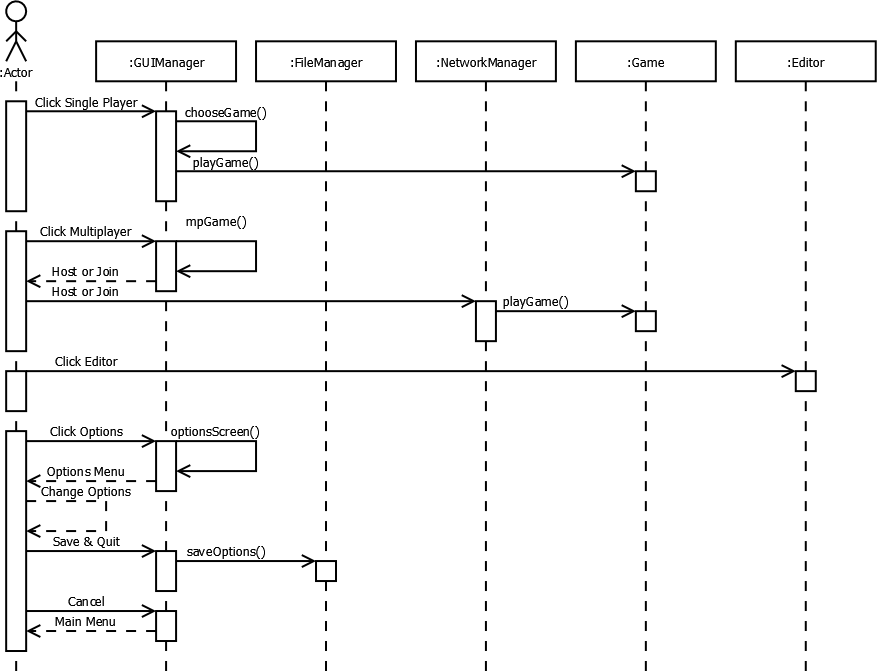
\includegraphics[width=1\linewidth]{Anttris_GUISequence.png}
\end{frame}

\begin{frame}
    \frametitle{GUI} % CHRIS
    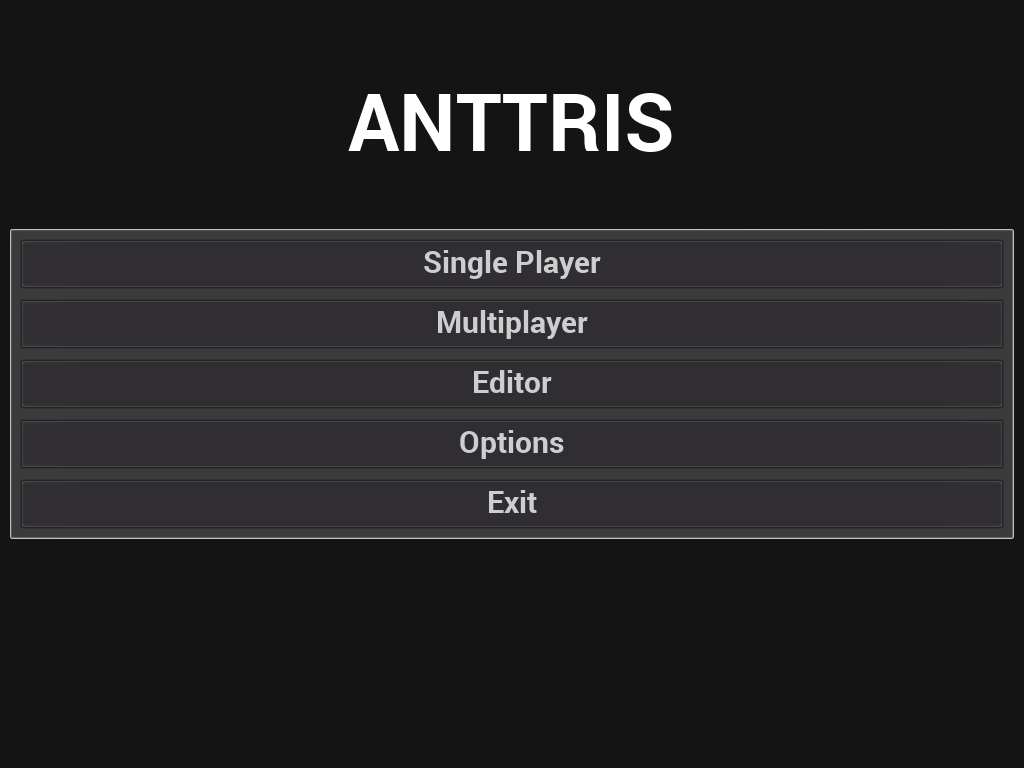
\includegraphics[width=1\linewidth]{Anttris_MainMenu.png}
\end{frame}

\begin{frame}
    \frametitle{Data Manager} % CHRIS
    \begin{itemize}
	\item Serialize Data
	\pause \item Save / Load Options
	\pause \item Save / Load Puzzles
	\end{itemize}
\end{frame}

\begin{frame}
    \frametitle{Editor} % HUGO
    \begin{itemize}
        \item Add/replace/remove different block types
        \item Load/save
        \pause \item Mobile friendly interface
        \pause \item Layer management: create random, remove current (Stretch goal)
    \end{itemize}
\end{frame}

\begin{frame}
    \frametitle{Generator} % CHRIS
    The Problem:
    \begin{itemize}
	\pause \item Need to generate puzzles
	\pause \item Need to be solvable
	\pause \item Need to follow the rules
	\end{itemize}

	\pause The Solution:
	\begin{itemize}
	\pause \item Generate all positions
	\pause \item Randomize
	\pause \item Assign based on position
	\pause \item Randomize pairs
	\end{itemize}
\end{frame}

\begin{frame}
    \frametitle{Solver} % CHRIS
    The Problem:
    \begin{itemize}
	\pause \item Need to check for solutions
	\pause \item Check random puzzles
	\pause \item Check puzzles from the editor
	\end{itemize}

	\pause The Solution:
	\begin{itemize}
	\pause \item Pull out pair blocks
	\pause \item Make sure all pair blocks have a pair
	\pause \item Check if the pair is on the same layer
	\end{itemize}
\end{frame}

\begin{frame}
    \frametitle{Networking} % SKYLER
    \begin{itemize}
        \pause \item Multiplayer
        \pause \item P2P
        \begin{itemize}
            \pause \item Non-random Opponents
            \pause \item Network Information
        \end{itemize}
        \pause \item Key Events
        \begin{itemize}
            \pause \item Start of Game
            \pause \item Transform Puzzle
            \pause \item Select Blocks
            \pause \item Game End
	\end{itemize}
    \end{itemize}
\end{frame}

\begin{frame}
    \frametitle{Rules} % CHRIS
    \begin{itemize}
	\item The puzzle grid
	\pause \item Pair blocks
	\pause \item Laser blocks
	\pause \item Wild blocks
	\pause \item Score
	\end{itemize}

\end{frame}

\begin{frame}
    \frametitle{Grand Summary} % BENJI
\end{frame}


\section{Implementation}
\begin{frame}
  \frametitle{Approach} % Hugo? idk
\end{frame}

\begin{frame}
    \frametitle{Godot} % HUGO
    % blank on purpose
\end{frame}

\begin{frame}[fragile]
    \frametitle{GD Script} % HUGO
    \begin{itemize}
        \pause \item Domain specific language
        \pause \item Object oriented, python-like
        \pause \item Dynamic, bugs easy to introduce
        \pause \item Example: methods passed as (object, string) tuples

        \pause \item Files are classes

        \begin{Verbatim}[numbers=left]
             extends ``Food.gd''

             func fry():
                 return self.fried()

             class GrillFuel:
                 ...
        \end{Verbatim}

        \pause \item Tightly integrated with all of Godot's C++ classes. Fast
            where it counts.
    \end{itemize}
\end{frame}

\begin{frame}
    \frametitle{Godot} % HUGO
    \begin{itemize}
    \item GoDot was easy to learn.
    \pause \item Library consisting of 400+ classes, less so
    \pause \item Limited use of the neat GUI interface, binary files don't
        agree with Github
    \end{itemize}

\end{frame}

\begin{frame}
    \frametitle{Code Overview} % line counts..., UML
\end{frame}


\section{Workflow} % SEAN
\begin{frame}
    \frametitle{Our Workflow}
    \begin{itemize}
    		\pause \item We used Github as our source control.
    		\pause \item To facilitate an agile workflow we used Zenhub.
    		\begin{itemize}
    		\pause \item Zenhub integrates a Scrum board right in Github.
    		\pause \item We set out to use certain parts of Scrum, but we're students!
    		\pause \item Which means, we didn't always adhere to the rules.
    		\end{itemize}
    		\pause \item Continuous Integration
    		\begin{itemize}
    			\pause \item Travis CI. It's awesome and everyone should try it!
    			\pause \item Not to mention free for open source projects.
    		\end{itemize}
    		\pause \item Branches
    		\begin{itemize}
    			\pause \item We used branches and pull requests to merge changes.
    			\pause \item This facilites easy code reviews before things get broken!
    		\end{itemize}
    \end{itemize}
\end{frame}

\begin{frame}
    \frametitle{Workflow, Continued}
    \begin{itemize}
    		\pause \item Unit testing
    		\begin{itemize}
    			\pause \item We used the [G]odot [U]nit [T]esting framework, aka GUT.
    			\pause \item This works nicely with Travis, thanks to a Python script Hugo wrote to catch return values and report on unit test results.
    			\pause \item This project is hosted on Bitbucket at {\url https://bitbucket.org/bitwes/gut/overview}.
    		\end{itemize}
	\end{itemize}
\end{frame}

\begin{frame}
    \frametitle{Project Pace} % BENJI
\end{frame}

\begin{frame}
  \frametitle{What we learned} % SKYLER
\end{frame}

%% From Dr Shin's slides
\begin{frame}
  \frametitle{Demo} % ALL, BRING ANDROIDS, LAPTOPS (OSX, WINDOWS, LINUX)
\end{frame}
%% ------ %%

\end{document}
